%%%%%%%%%%%
%% Home work template for Graduate School
%% Author : Thamme Gowda N.
%% Originally from  https://github.com/thammegowda/hw-tex-templ
%%%%%%%%%%%%%%

\documentclass[letterpaper,doc,notimes]{apa6}
%%\documentclass[tikz]{standalone}
\usepackage{tikz}
%Required by APA6 package
\usepackage[normalem]{ulem}
\usepackage[english]{babel}
\usepackage[utf8x]{inputenc}
\usepackage{amsmath}
\usepackage{amsfonts}
\usepackage{graphicx}
\usepackage{adjustbox}

%Oft-used, oft-abused
\usepackage{afterpage}
\usepackage{booktabs}
\usepackage{caption}
\usepackage{censor}
\usepackage{color}
\usepackage{csquotes}
\usepackage{enumitem}
\usepackage{float}
\usepackage{hyperref}
\usepackage{lmodern}
%\usepackage{media9}
\usepackage{multirow}
\usepackage{outlines}
\usepackage{pdfpages}
\usepackage{placeins}
\usepackage{soul}
\usepackage{tabularx}
\usepackage[colorinlistoftodos]{todonotes}
\usepackage{xcolor}
\usepackage{mathtools}
\graphicspath{ {images/}}

\usepackage{sectsty}
\sectionfont{\fontsize{16}{15}\selectfont}


\setenumerate[1]{label=\Roman*.}
\setenumerate[2]{label=\Alph*.}
\setenumerate[3]{label=\roman*.}
\setenumerate[4]{label=\alph*.}

% break page where ever is required
\allowdisplaybreaks

\title{ \textbf{ USC CSCI 567 HOMEWORK 2 SOLUTIONS} }
\shorttitle{USC CSCI567 FALL16 HW2}
\author{\textsc{ThammeGowda Narayanaswamy}}
\affiliation{ tnarayan@usc.edu \\ ID : 2074-6694-39 \\ Department of Computer Science \\ Viterbi School of Engineering \\ University of Southern California \\ Los Angeles, CA 
	}



%\note{September 13, 2016}
\note{\today}
\note{ Collaborators : \\ Ishan Alok (ialok@usc.edu)}

\authornote{Produced for Fall 2016 session of CSCI 567, ``Machine Learning'', taught by Dr. Yan Liu at the University of Southern California}


\begin{document}

\maketitle
\newpage

\section{1. LOGISTIC REGRESSION}
\subsection{a. Negative Log Likelihood of Binary Logistic Regression}
The sigmoid-logistic function, defined by $\sigma(x) = \frac{1}{1 + e^{-x}}$ \\
Given that the dataset has $n$ examples, namely $\{(x_1,y_1), (x_2,y_2),... (x_n,y_n)\}$ \\
Where the class labels, $y_i = \{0, 1\}$  and $x_i$ $ \in \mathbb{R}^D$ \\
Let $w$ $ \in \mathbb{R}^D$ parameter which has to be learned by logistic regressor for optimal classification.\\
The probability estimation is defined by $P(Y=y_i|X=x_i) = \sigma(w^Tx_i) $. \\
The negative log likelihood is defined by:
\begin{align*}
		L(w) = & -log\bigg(\prod_{i=1}^{n} P(Y=y_i|X=x_i) \bigg) \\
		= & -\sum_{i=1}^{n}\bigg( log\big( P(Y=y_i|X=x_i) \big)\bigg) \\
		= & -\sum_{i=1}^{n}\bigg( log\big( P(Y=1|X=x_i)P(Y=0|X=x_i) \big)\bigg) \\
		= & -\sum_{i=1}^{n}\bigg( log\big[ \sigma(w^Tx_i)^{y_i} \times (1 - \sigma( w^Tx_i))^{1 - y_i} \big]\bigg) \\
		= & -\sum_{i=1}^{n}\bigg( y_i log\big[ \sigma(w^Tx_i) \big] + (1 - y_i ) log\big[ 1 - \sigma(w^Tx_i) \big]\bigg) \\
	%%	& w^Tx \text{ can also be expressed as sum of products, } \sum_{j}^{D} w_jx_j\\
\end{align*}

\section{1.b Find the update rule using gradient descent}
From the previous section, we have 
\begin{align*}
	E(w) = & \mathcal{L}(w) = -\sum_{i=1}^{n}\bigg( y_i log\big[ \sigma(w^Tx_i) \big] + (1 - y_i ) log\big[ 1 - \sigma(w^Tx_i) \big]\bigg) \\
	& \text{we know that $w$ is a multivariate function of variables } \{w_0, w_1, w_2, ....w_d\} \\
	&  w^Tx \text{ can also be expressed as sum of products, } \sum_{j}^{d} w_jx_j\\
	= & -\sum_{i=1}^{n}\bigg( y_i log\big[ \sigma(\sum_{j}^{d} w_jx_j) \big] + (1 - y_i ) log\big[ 1 - \sigma(\sum_{j}^{d} w_jx_j) \big]\bigg) \\
	& \text{We find the gradient of $E(w)$ w.r.t variable $w_j$ for $j = 0, 1, ...d $} \\ 
 \dfrac{\partial E(w)}{\partial w_j} = & -\sum_{i=1}^{n} \bigg(
			  y_i \dfrac{\partial}{\partial w_j} log\big[ \sigma(\sum_{j}^{d} w_jx_j) \big] 
			  + (1 - y_i ) \dfrac{\partial}{\partial w_j} log\big[ 1 - \sigma(\sum_{j}^{d} w_jx_j) 
		\big]\bigg) \\ 
		\\
\end{align*}
Let us evaluate the derivatives individually
\begin{align*}
\dfrac{\partial}{\partial w_j} log\big[ \sigma(\sum_{j}^{d} w_jx_j) \big]  = &
		 \dfrac{\partial}{\partial w_j} log\big[  \frac{1}{1 + e^{-\sum_{j}^{d} w_jx_j} } \big]\\
	= &  (1 + e^{-\sum_{j}^{d} w_jx_j}) \times \frac{-1}{(1 + e^{-\sum_{j}^{d} w_jx_j})^2} \times e^{-\sum_{j}^{d} w_jx_j} \times (-x_j) \\
	= &  \frac{1}{1 + e^{-\sum_{j}^{d} w_jx_j}} \times e^{-\sum_{j}^{d} w_jx_j} \times (x_j) \\
	= & x_j \times [1 - \sigma(\sum_{j}^{d} w_jx_j)] \\
	= & x_j \times [1 - \sigma(w^Tx)] \\
	\\
\dfrac{\partial}{\partial w_j} log\big[ 1 - \sigma(\sum_{j}^{d} w_jx_j) = &
	\dfrac{\partial}{\partial w_j} log\big[ 1 - \frac{1}{1 + e^{-\sum_{j}^{d} w_jx_j} } \big] \\
	= &  \frac{1}{1 - \frac{1}{1 + e^{-\sum_{j}^{d} w_jx_j}}} \times \frac{-1 \times -1 }{(1 + e^{-\sum_{j}^{d} w_jx_j})^2} \times e^{-\sum_{j}^{d} w_jx_j} \times (-x_j) \\
	= & -x_j \times \sigma(w^Tx) \\ 
\end{align*}

Putting the above two values in the original equation, we have:
\begin{align*}
\dfrac{\partial E(w)}{\partial w_j} = & -\sum_{i=1}^{n} \bigg(
	 y_i \dfrac{\partial}{\partial w_j} log\big[ \sigma(\sum_{j}^{d} w_jx_j) \big] 
	 + (1 - y_i ) \dfrac{\partial}{\partial w_j} log\big[ 1 - \sigma(\sum_{j}^{d} w_jx_j) 
	 \big]\bigg) \\
	 = & -\sum_{i=1}^{n} \bigg(	x_j y_i (1 - \sigma(w^Tx)) - (1 - y_i ) x_j \sigma(w^Tx) \bigg) \\
\end{align*}

The update rule using gradient descent is given by,

\begin{equation*}
	w_j = w_j - \alpha \dfrac{\partial E(w)}{\partial w_j}
\end{equation*}
{Where $\alpha$ is the learning or step rate.

Provided proper learning rate $\alpha$, Gradient descent optimizer converges to global minimum for all convex functions. So, to test the convexity of the negative log likelihood function, let us compute second order derivatives.

\begin{align*}
\dfrac{\partial^2 E(w)}{\partial w_j^2} = & \dfrac{\partial}{\partial w_j} \dfrac{\partial E(w)}{\partial w_j} \\
	= & -\sum_{i=1}^{n} \dfrac{\partial}{\partial w_j} \bigg(	x_j y_i (1 - \sigma(w^Tx)) - (1 - y_i ) x_j \sigma(w^Tx) \bigg) \\
	= & -\sum_{i=1}^{n} \bigg( x_j y_i (- \dfrac{\partial}{\partial w_j} \sigma(w^Tx)) - (1 - y_i ) x_j \dfrac{\partial}{\partial w_j} \sigma(w^Tx) \bigg) \\
	= & -\sum_{i=1}^{n} \bigg( x_j y_i (-x_j \sigma(w^Tx) (1 - \sigma(w^Tx))) - (1 - y_i ) x_j x_j  \sigma(w^Tx) (1 - \sigma(w^Tx)) \bigg) \\
	= & -\sum_{i=1}^{n} \bigg( [ -y_i - (1 - y_i ) ] x_j^2 \sigma(w^Tx) (1 - \sigma(w^Tx)) \bigg)  \\
	= & \sum_{i=1}^{n} \bigg([ y_i + 1 - y_i ) ] x_j^2 \sigma(w^Tx) (1 - \sigma(w^Tx)) \bigg)  \\
	= & \sum_{i=1}^{n} \bigg( x_j^2 \sigma(w^Tx) (1 - \sigma(w^Tx)) \bigg) \\
\end{align*}

We know that, $\sigma(w^Tx)$ is the $(P(Y=1|X=x))$ which is  >= 0, also, $(1 - \sigma(w^Tx))$ is the $(P(Y=0|X=x))$ which is also >= 0. \\
Thus $\dfrac{\partial^2 E(w)}{\partial w_j^2} >= 0 $. \\
Therefore, negative log likelihood function is convex.  Hence Gradient descent finds the global minimum.

\subsection{c. Multi class logistic regression model's Negative log likelihood}

Given that we have `K` classes, namely k=\{1,2,3,4,...K\}.

We know that the posterior probability of each class sums up to 1.
\begin{align*}
	\sum_{k=1}^{K} P(Y = k | X = x_i) = 1
\end{align*}

To reduce the number of required parameters, we can use the above result to precisely compute the probability of a class if we know rest all other classes.
\begin{align*}
	P(Y = K | X = x_i) = 1 - \sum_{k=1}^{K-1} P(Y = k | X = x_i)
\end{align*}

Let us define an Indicator function
 $I(y_i = k)$ which hs value $1$ when $y_i = k$, and has $0$ if $y_i \ne k$ 

For a dataset of $N$ examples, the likelihood of this multi class classifier (using fewer parameters ) is defined by
\begin{align*}
	l(w) = \prod_{n=1}^{N} \prod_{k=1}^{K-1} P(Y = y_n | X = x_n ) ^ {I(y_n=k)} (1 - \sum_{k=1}^{K-1} P(Y = y_n | X = x_n ) ^ {I(y_n=k)})
\end{align*}
We can simplify this equation without adding any additional parameters but setting $W_K=0$ as given in the problem description.

\begin{align*}
	\ell (w) = & \prod_{n=1}^{N} \prod_{k=1}^{K} P(Y = y_n | X = x_n )^{I(y_n = k)} & &
\end{align*}
The negative log likelihood is given by
\begin{align*}
  \mathcal{L}(w) = & - log \bigg [ \prod_{n=1}^{N} \prod_{k=1}^{K} P(Y = y_n | X = x_n )^{I(y_n = k)} \bigg]  & & \\
	   = & - \sum_{n=1}^{N} \sum_{k=1}^{K} log P(Y = y_n | X = x_n ) ^{I(y_n = k)}  & & \\
	   = & - \sum_{n=1}^{N} \sum_{k=1}^{K} log \bigg[ \frac{e^{w_k^Tx_n}}{1 + \sum_{t=1}^{K} e^{w_t^Tx_n}}  \bigg]^{I(y_n = k)}  & & \\
	   = & - \sum_{n=1}^{N} \sum_{k=1}^{K} I(y_n = k) \bigg[ w_k^Tx_n - log [1 +  \sum_{t=1}^{K} e^{w_t^Tx_n} ] \bigg]  & & \\
\end{align*}

\subsection{d. Gradient descent update rule}
Let us consider the final equation of previous section.
The $\mathcal{L}$ is a multivariate function with variables $w_i$ for i = 1, 2,3, ... K . \\

\begin{align*}
	\mathcal{L}(w_1, w_2, ...w_K ) = & - \sum_{n=1}^{N} \sum_{k=1}^{K} I(y_n = k) \bigg[ w_k^Tx_n - log [1 +  \sum_{t=1}^{K} e^{w_t^Tx_n} ] \bigg] 
\end{align*}
The first order derivative of $\mathcal{L}$ w.r.t $w_i$ is:

\begin{align*}
\frac{\partial \mathcal{L}}{\partial w_i} = & - \frac{\partial }{\partial w_i } \sum_{n=1}^{N} \sum_{k=1}^{K} I(y_n = k) \bigg[ w_k^Tx_n - log [1 +  \sum_{t=1}^{K} e^{w_t^Tx_n} ] \bigg ] \\
= & - \sum_{n=1}^{N} \sum_{k=1}^{K} I(y_n = k) \bigg[ x_{ni}  - \frac{1}{1 + \sum_{t=1}^{K} e^{w_t^Tx_n}} \times \sum_{t=1}^{K} e^{w_t^Tx_n} \times x_{ni} \bigg] \\
& \text{$x_n$ is a vector of all atttributes of $n^{th}$ example} 
\\ & \text{where as $x_{ni}$ is a scalar from $i^{th}$ attribute of $n^{th}$ example} \\
\\
= & - \sum_{n=1}^{N} \sum_{k=1}^{K} x_{ni} I(y_n = k) \bigg[ 1  - \frac{\sum_{t=1}^{K} e^{w_t^Tx_n}}{1 + \sum_{t=1}^{K} e^{w_t^Tx_n}}  \bigg] \\
\frac{\partial \mathcal{L}}{\partial w_i} = & - \sum_{n=1}^{N} \sum_{k=1}^{K} x_{ni} I(y_n = k) \bigg[ \frac{1}{1 + \sum_{t=1}^{K} e^{w_t^Tx_n}}  \bigg] \\
\end{align*}
The update rule for gradient descent optimizer with step rate $\alpha$ is: 
\begin{align*}
	w_i = & w_i - \alpha \frac{\partial \mathcal{L}}{\partial w_i} \\
	& \text{for all } i = \{1, 2, 3,...K\}
\end{align*}



%%%%%%%%%%%%%%%%%%%%%%%%%%%%%%%%%%%%%%%%%%%%%%%%%%%%%%%%%%%%%%%%%%%%%%%%
\section{2. LINEAR/GAUSSIAN DISCRIMINANT ANALYSIS}

\subsection{a. Log likelihood and MLE estimates}
Given:

The dataset $\mathcal{D}$ has $N$ examples, $\{(x_1,y_1), (x_2, y_2), ...(x_N, y_N)\}$

There are two classes $y_n = \{1, 2\} $

$P(y_n = 1) = p_1$ and $P(y_n = 2) = p_2$

$P(x_n | y_n=1) = \frac{1}{\sqrt{2\pi } \cdot \sigma_1} \exp(-\frac{(x_n-\mu_1)^2}{2\sigma_1^2})$

$P(x_n | y_n=2) = \frac{1}{\sqrt{2\pi } \cdot \sigma_2} \exp(-\frac{(x_n-\mu_2)^2}{2\sigma_2^2})$ \\

Let us define Indicator functions $I(y_n=1)$ and $I(y_n=2)$


\paragraph{Log Likelihood}
The log likelihood is defined by
\begin{align*}
\mathcal{L} = & ln \bigg[ \prod_{n=1}^{N} P(x_n, y_n) \bigg] \\
	= &  \ln \bigg[ \prod_{n=1}^{N} P(x_n, y_1)^{I(y_n=1)} \times P(x_n, y_1)^{I(y_n=2)} \bigg] \\
	= & \ln \bigg[ \prod_{n=1}^{N} P(x_n, y_1)^{I(y_n=1)} \times P(x_n, y_1)^{I(y_n=2)} \bigg] \\
	= &  \sum_{n=1}^{N}\bigg[ ln P(x_n, y_1)^{I(y_n=1)} + ln P(x_n, y_1)^{I(y_n=2)} \bigg] \\
	= &  \sum_{n=1}^{N}\bigg[ I(y_n=1) \ln \big[ p_1 \times \frac{1}{\sqrt{2\pi } \cdot \sigma_1} \exp(-\frac{(x_n-\mu_1)^2}{2\sigma_1^2}) \big] 
			 + I(y_n=2) \ln \big[ p_2 \times \frac{1}{\sqrt{2\pi } \cdot \sigma_2} \exp(-\frac{(x_n-\mu_2)^2}{2\sigma_2^2}) \big] \bigg]  \\
	= & \sum_{n=1}^{N}\bigg[
		I(y_n=1)\big[ \ln(p_1) -\frac{1}{2}\ln(2\pi) - \ln(\sigma_1) - \frac{1}{2\sigma_1^2} (x_n-\mu_1)^2 \big] \\
		 & \indent  + 
		I(y_n=2)\big[ \ln(p_2) -\frac{1}{2}\ln(2\pi) - \ln(\sigma_2) - \frac{1}{2\sigma_2^2} (x_n-\mu_2)^2 \big] \bigg] \\
\end{align*}

The above likelihood expression is a multivariate function with parameters $(p1, p2, \mu_1, \mu_2, \sigma_1, \sigma_2 )$.
From a fundamental law of probability, we know that
\begin{align*}
	p_1 + p_2 = & 1\\
	 p_2 = & 1 - p_1 \\
	 p_1 = & 1 - p_2
\end{align*}
Thus,
\begin{multline}
	\mathcal{L} (p1, \mu_1, \mu_2, \sigma_1, \sigma_2 )	=  \sum_{n=1}^{N}\bigg[
	I(y_n=1)\big[ \ln(p_1) -\frac{1}{2}\ln(2\pi) - \ln(\sigma_1) - \frac{1}{2\sigma_1^2} (x_n-\mu_1)^2 \big] \\
		\indent \indent \indent + 
	I(y_n=2)\big[ \ln(1 - p_1) -\frac{1}{2}\ln(2\pi) - \ln(\sigma_2) - \frac{1}{2\sigma_2^2} (x_n-\mu_2)^2 \big] \bigg] \\
\end{multline}
Let us find an estimate of these parameters using maximum likelihood estimator method.\\\
To find an estimate of $p_1$, we solve $\frac{\partial \mathcal{L} }{\partial p_1} = 0$
\begin{align*}
\frac{\partial \mathcal{L} }{\partial p_1} =& 0 \\
\sum_{n=1}^{N}\big[I(y_n=1)\frac{1}{p_1}  + I(y_n=2)\frac{1}{1-p_1} \times(-1) \big]  =& 0 \\ 
\frac{1}{p_1} \sum_{n=1}^{N} I(y_n=1)  - \frac{1}{1-p_1} \sum_{n=1}^{N} I(y_n=2) =& 0 \\ 
(1-p_1) \sum_{n=1}^{N} I(y_n=1)  - p_1 \sum_{n=1}^{N} I(y_n=2) =& 0 \\ 
p_1 =&  \frac{\sum_{n=1}^{N} I(y_n=1) }{\sum_{n=1}^{N} I(y_n=1) + \sum_{n=1}^{N} I(y_n=2)}\\ 
\implies p_1^* =&  \frac{\sum_{n=1}^{N} I(y_n=1) }{N} \\ 
\text{Similarly,} \\
1 - p_1 =& 1 - \frac{\sum_{n=1}^{N} I(y_n=1) }{N} = \frac{N - \sum_{n=1}^{N} I(y_n=1) }{N} \\ 
\implies p_2^* =&  \frac{\sum_{n=1}^{N} I(y_n=2) }{N} \\ 
\end{align*}

To find an estimate of $\mu_1$ when $\mathcal{L}$ is maximum, let us solve for $\frac{\partial \mathcal{L} }{\partial \mu_1} = 0$
\begin{align*}
\frac{\partial \mathcal{L} }{\partial \mu_1} =& 0 \\
	\sum_{n=1}^{N} I(y_n=1) \times \frac{-1}{2\sigma_1} \times 2 \times (x_n - \mu_1) \times -1 =& 0 \\
	\sum_{n=1}^{N} I(y_n=1) \times (x_n - \mu_1) =& 0 \\
		\sum_{n=1}^{N} I(y_n=1) x_n =&  \sum_{n=1}^{N} I(y_n=1) \mu_1 \\
				\sum_{n=1}^{N} I(y_n=1) x_n =& \mu_1 \sum_{n=1}^{N} I(y_n=1) \\
				\frac{ \sum_{n=1}^{N} I(y_n=1) x_n } {\sum_{n=1}^{N} I(y_n=1)}=& \mu_1  \\
				\implies \mu_1^* = & \frac{ \sum_{n=1}^{N} I(y_n=1) x_n } {\sum_{n=1}^{N} I(y_n=1)}  \\
		\text{We already know that, }  p_1 \times N = \sum_{n=1}^{N} I(y_n=1) & \\
	 \implies \mu_1^* = & \frac{ \sum_{n=1}^{N} I(y_n=1) x_n } {p_1 N} \\
	 \\
 \text{$\mu_2$ when $\mathcal{L}$ is maximum can be estimated by solving} & \\ \frac{\partial \mathcal{L} }{\partial \mu_2} = &0 \\
	 \implies \mu_2^* = & \frac{ \sum_{n=1}^{N} I(y_n=2) x_n } {\sum_{n=1}^{N} I(y_n=2)}  \\
	 	  = & \frac{ \sum_{n=1}^{N} I(y_n=2) x_n } {p_2 N} \\
\end{align*}

To find an estimate of $\sigma_1$ when $\mathcal{L}$ is maximum, let us solve
\begin{align*}
	\frac{\partial \mathcal{L} }{\partial \sigma_1} = &0  \\
	\sum_{n=1}^{N} I(y_n=1) \big[ -\frac{1}{\sigma_1} -\frac{(x_n - \mu_1)^2}{2} \times \frac{-2}{\sigma^3} \big] =& 0 \\
	\sum_{n=1}^{N} I(y_n=1) \big[ -\sigma_1^2 + (x_n - \mu_1)^2 \big] =& 0 \\
	\sigma_1^2 \sum_{n=1}^{N} I(y_n=1) =& \sum_{n=1}^{N} I(y_n=1) (x_n - \mu_1)^2 \\
    \sigma_1^2 =& \frac{ \sum_{n=1}^{N} I(y_n=1) (x_n - \mu_1)^2 }{\sum_{n=1}^{N} I(y_n=1)}\\
  \implies \sigma_1^* =& \sqrt{ \frac{ \sum_{n=1}^{N} I(y_n=1) (x_n - \mu_1)^2 }{\sum_{n=1}^{N} I(y_n=1)} } = \sqrt{ \frac{ \sum_{n=1}^{N} I(y_n=1) (x_n - \mu_1)^2 }{p_1 N} } \\
\end{align*}

Similarly, to find an estimate of $\sigma_2$ when $\mathcal{L}$ is maximum, let us solve

\begin{align*}
\frac{\partial \mathcal{L} }{\partial \sigma_2} = &0  \\
\implies \sigma_2^* =& \sqrt{ \frac{ \sum_{n=1}^{N} I(y_n=2) (x_n - \mu_2)^2 }{\sum_{n=1}^{N} I(y_n=2)} } = \sqrt{ \frac{ \sum_{n=1}^{N} I(y_n=2) (x_n - \mu_2)^2 }{p_2 N} } \\
\end{align*}


\subsection{b. Reduction to Logistic Sigmoid function form}
Given :\\
\indent  There are two classes, $y_n = \{c_1, c_2\}$ \\
\indent  $P(x | y= c_1) = \mathcal{N}(\mu_1, \sum)$  \\
\indent  $P(x | y=c_2) = \mathcal{N}(\mu_2, \sum) $ \\

\noindent We know \\
\indent for $D$ variables, \\
\indent \indent $\mathcal{N}(\mu, \sum) = (2\pi)^{-D/2} \sum^{-1/2} \exp[-\frac{1}{2} (x-\mu)^T \space \sum^{-1} \space (x-\mu)]$

\noindent Goal: \\
\indent  To express $P(y=c_1|x) $ in logistic sigmoid form

\noindent Solution:
\begin{align*}
\text{Using the Bayes rule} & \\
	P(y =& c_1|x) = \frac{P(x | y=c1) P(y=c1)}{P(x)} \\
\text{Using the law of otal probability} \\
	P(y =& c_1|x) = \frac{P(x | y=c1) P(y=c1)}{P(x | y=c1) P(y=c1) + P(x | y=c2) P(y=c2)} \\
	P(y =& c_1|x) = \frac{1}{1 + \frac{ P(x | y=c2) P(y=c2)}{P(x | y=c1) P(y=c1)} } \\
\text{This is of form} \\
	P(y =& c_1|x) = \frac{1}{1 + f(x)} \\
\text{where } f(x) = & \frac{P(y=c2)}{P(y=c1)} \times \frac{P(x|y=c2) }{P(x|y=c1)} \\
	 = & \frac{P(y=c2)}{P(y=c1)} \times \frac{\mathcal{N}(\mu_2, \sum) }{\mathcal{N}(\mu_1, \sum)}
\end{align*}
Now, substituting the values in $f(x)$
\begin{align*}
f(x) = & \frac{P(y=c2)}{P(y=c1)} \times \frac{(2\pi)^{-D/2} \sum^{-1/2} \exp[-\frac{1}{2} (x-\mu_2)^T \space \sum^{-1} \space (x-\mu_2)] }  {(2\pi)^{-D/2} \sum^{-1/2} \exp[-\frac{1}{2} (x-\mu_1)^T \space \sum^{-1} \space (x-\mu_1)]}\\ 
  = & \frac{P(y=c2)}{P(y=c1)} \times \exp \bigg[\frac{1}{2}  \big[(x-\mu_1)^T \space \sum^{-1} \space (x-\mu_1) - (x-\mu_2)^T \space \sum^{-1} \space (x-\mu_2)  \big] \bigg] \\
  \\ 
&  \text{For the sake of similification, we can use the form, } x = \exp(\ln(x))\\ 
\exp(\ln(f(x))) = &\exp(\ln\bigg( \frac{P(y=c2)}{P(y=c1)} \times \exp \bigg[\frac{1}{2}  \big[(x-\mu_1)^T \space \sum^{-1} \space (x-\mu_1) - (x-\mu_2)^T \space \sum^{-1} \space (x-\mu_2)  \big] \bigg] \bigg)) \\
\\
f(x) = &\exp(\ln(\frac{P(y=c2)}{P(y=c1)}) + \frac{1}{2} \big[(x-\mu_1)^T \space \sum^{-1} \space (x-\mu_1) - (x-\mu_2)^T \space \sum^{-1} \space (x-\mu_2)  \big] ) \\
f(x) = &\exp( - \big(- \ln(\frac{P(y=c2)}{P(y=c1)}) + \frac{1}{2} \big[ (x-\mu_2)^T \space \sum^{-1} \space (x-\mu_2) - (x-\mu_1)^T \space \sum^{-1} \space (x-\mu_1)\big] \big)) \\
\end{align*}
This equation is of  form $\exp(-(\theta_0 + {\theta}^Tx))$
Where, $\theta_0$ is a scalar computed by - $\ln(\frac{P(y=c2)}{P(y=c1)}) $ \\
 and $\theta^Tx$ is another scalar computed by $\frac{1}{2} \big[(x-\mu_2)^T \space \sum^{-1} \space (x-\mu_2) - (x-\mu_1)^T \space \sum^{-1} \space (x-\mu_1)  \big]$, but $\theta$ and $x$ are vectors of $D$ dimensions.
 
 Substituting the value of $f(x)$ in the original equation above, we get:
\begin{align*}
	P(y =& c_1|x) = \frac{1}{1 + f(x)} 
		= \frac{1}{1 + exp(-(\theta_0 + \theta^Tx))} 
 \end{align*}
 The above expression is in logistic sigmoid form.
 However, we can further simplify the above equation by packing $\theta_0$ scalar parameter inside $\theta$ vector by inserting $1$ into $x$ vector at the corresponding dimension. \\
 \begin{equation}
	\implies 	P(y = c_1|x) = \frac{1}{1 + exp(-\theta^Tx)}
 \end{equation}
 where $\theta$ and $x$ are vectors of $D+1$ dimensions
 
 
 \section{4. Data Analysis}
 
 \subsection{a. Histograms of Attributes and the Target variable}

Here are the histograms of the dataset.\\
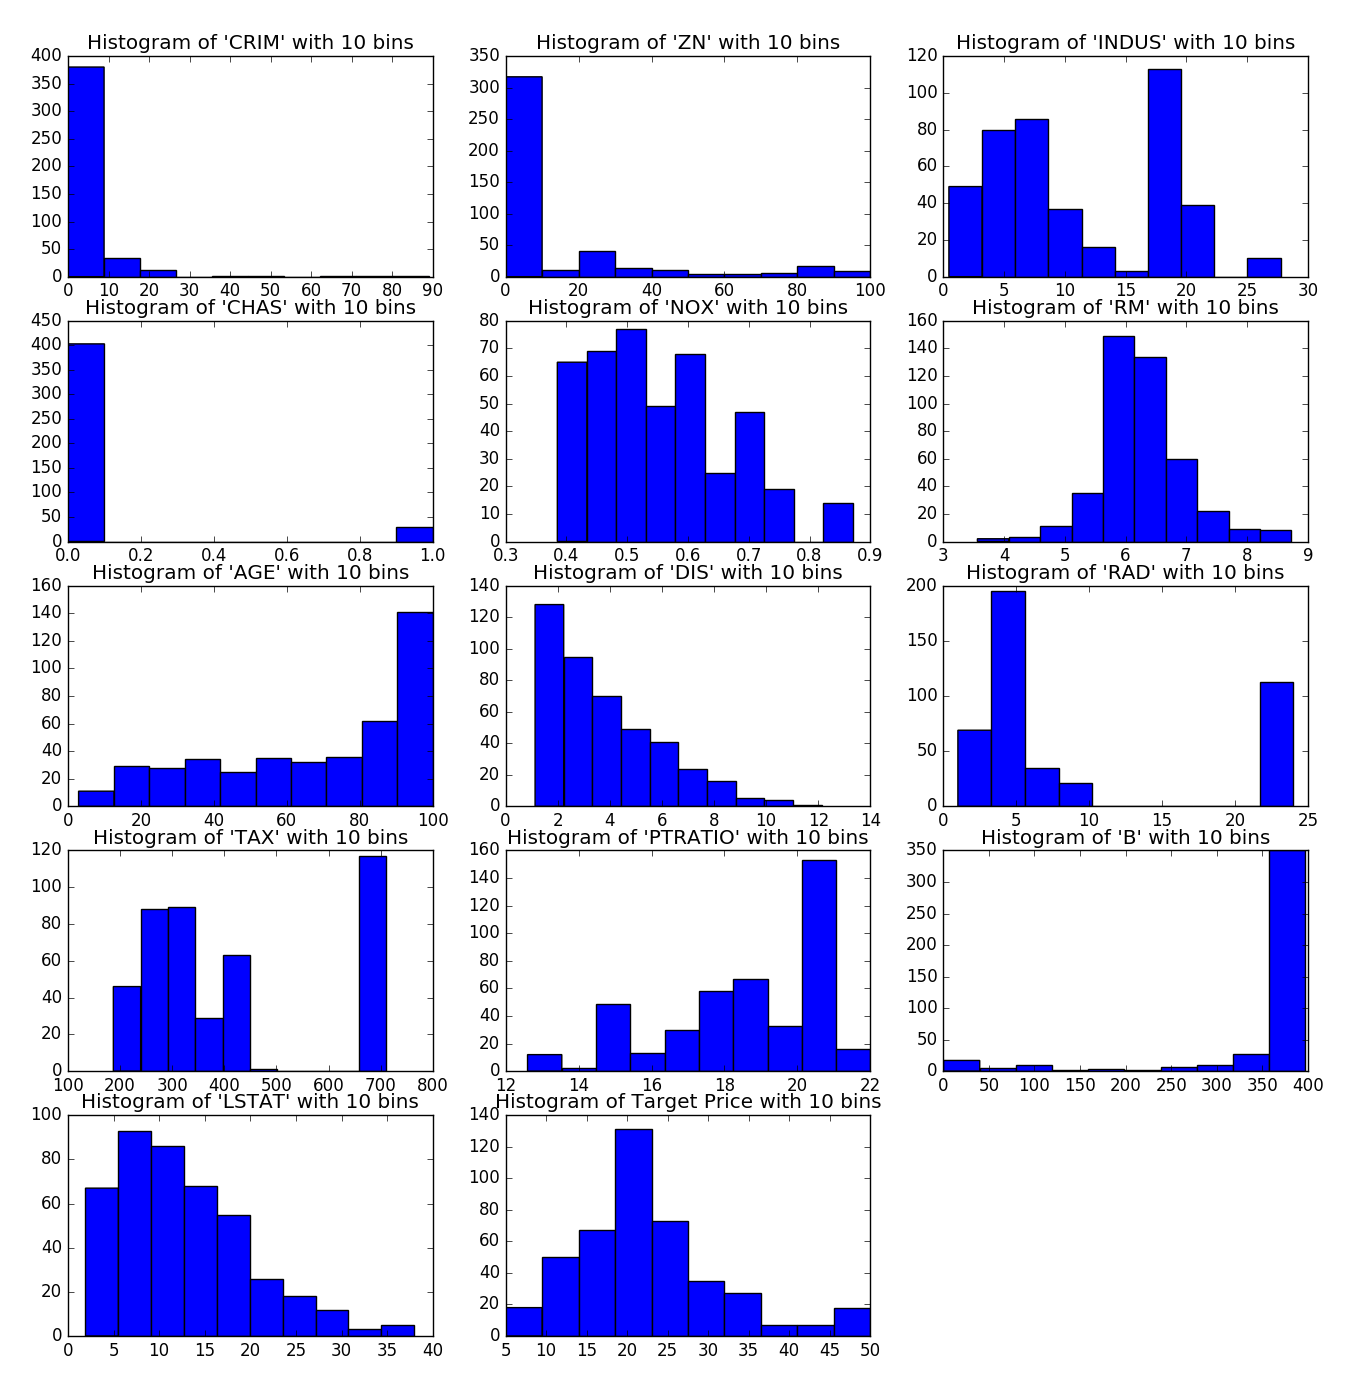
\includegraphics[scale=0.45]{Histograms}

Here are the correlations among the attributes:\\
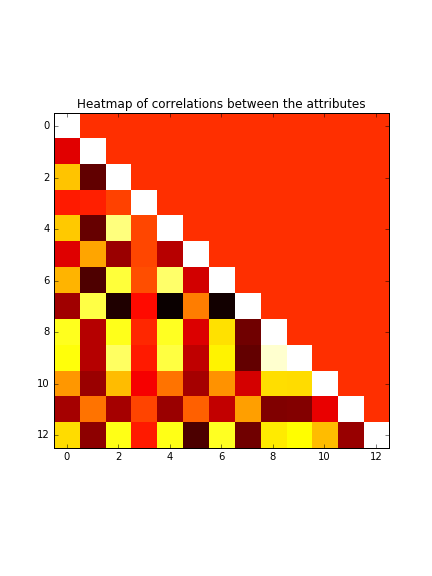
\includegraphics[scale=1]{correlation-heatmap}

\subsection{Program output}
\begin{verbatim}
$ python CSCI567_hw2_fall16.py 
 
The following parameters will be used for gradient descent optimizer:
 Learning rate= 0.001
 Convergence Tolerance= 0.005
 Max Iterations= 50000
 ##### 3.1 DATA ANALYSIS / EXPLORATION 
 Feature Names:
 0
 0      CRIM
 1        ZN
 2     INDUS
 3      CHAS
 4       NOX
 5        RM
 6       AGE
 7       DIS
 8       RAD
 9       TAX
 10  PTRATIO
 11        B
 12    LSTAT
 Dataset shape: (506, 13) (506, 1)
 Test shape: (73, 13) (73, 1)
 Train shape: (433, 13) (433, 1)
 Correlations between the attributes:
 0         1         2         3         4         5         6   \
 0   1.002315  0.000000  0.000000  0.000000  0.000000  0.000000  0.000000   
 1  -0.197276  1.002315  0.000000  0.000000  0.000000  0.000000  0.000000   
 2   0.396280 -0.537783  1.002315  0.000000  0.000000  0.000000  0.000000   
 3  -0.054158 -0.038522  0.050507  1.002315  0.000000  0.000000  0.000000   
 4   0.410524 -0.525903  0.769347  0.065319  1.002315  0.000000  0.000000   
 5  -0.206593  0.314229 -0.387829  0.066559 -0.308899  1.002315  0.000000   
 6   0.351814 -0.586247  0.654674  0.081180  0.734113 -0.239191  1.002315   
 7  -0.370380  0.672366 -0.713743 -0.097458 -0.771612  0.209400 -0.750088   
 8   0.607248 -0.317635  0.597033 -0.021546  0.611365 -0.211677  0.470596   
 9   0.567033 -0.318496  0.722513 -0.051311  0.668685 -0.288305  0.520563   
 10  0.279365 -0.383817  0.376030 -0.145421  0.183605 -0.356928  0.264867   
 11 -0.358765  0.180031 -0.360012  0.054895 -0.386504  0.134887 -0.284053   
 12  0.456168 -0.422381  0.591894 -0.057371  0.591094 -0.597977  0.608152   
 
 7         8         9         10        11        12  
 0   0.000000  0.000000  0.000000  0.000000  0.000000  0.000000  
 1   0.000000  0.000000  0.000000  0.000000  0.000000  0.000000  
 2   0.000000  0.000000  0.000000  0.000000  0.000000  0.000000  
 3   0.000000  0.000000  0.000000  0.000000  0.000000  0.000000  
 4   0.000000  0.000000  0.000000  0.000000  0.000000  0.000000  
 5   0.000000  0.000000  0.000000  0.000000  0.000000  0.000000  
 6   0.000000  0.000000  0.000000  0.000000  0.000000  0.000000  
 7   1.002315  0.000000  0.000000  0.000000  0.000000  0.000000  
 8  -0.498835  1.002315  0.000000  0.000000  0.000000  0.000000  
 9  -0.535925  0.913672  1.002315  0.000000  0.000000  0.000000  
 10 -0.236001  0.463870  0.457994  1.002315  0.000000  0.000000  
 11  0.296206 -0.452862 -0.449102 -0.177750  1.002315  0.000000  
 12 -0.498400  0.497685  0.545339  0.374000 -0.391823  1.002315 

 Magnitude of Correlation with the target 
 ('CRIM', 0.38859443435207547)
 ('ZN', 0.36382754420139768)
 ('INDUS', 0.48418563338201681)
 ('CHAS', 0.20407144132697344)
 ('NOX', 0.4258130776462164)
 ('RM', 0.69252269454509585)
 ('AGE', 0.39108230278590012)
 ('DIS', 0.25300487309124547)
 ('RAD', 0.38638415658601943)
 ('TAX', 0.46993468487617812)
 ('PTRATIO', 0.5064403651254078)
 ('B', 0.34422912357951185)
 ('LSTAT', 0.74168271373323336)
 ##### Generating Histograms
 
 
 ###### 3.2 a LINEAR REGRESSION ALGORITHM
 Using analytical optimizer
 W= [ 22.46351039  -0.9673241    1.04542152  -0.17351707   0.92139354
 -1.6205974    2.72573311  -0.26723668  -3.11240878   2.48363548
 -1.91078756  -1.88799963   0.82940209  -3.67532974]
 Train MSE:: 20.950144508 	Test MSE:: 28.4179164975
 Using gradient_desc optimizer
 W= [ 22.46351039  -0.93347984   0.97861438  -0.35174534   0.94966261
 -1.54772785   2.76534798  -0.30369741  -3.0952704    2.03099152
 -1.41039412  -1.86141796   0.82666393  -3.65780415]
 Train MSE:: 20.9818495194 	Test MSE:: 28.7478497502
 
 
 ##### 3.2 b RIDGE REGRESSION########
 
 Lambda		Train MSE		Test MSE
 0.01		21.0581242724		28.8462622276
 0.1		25.8139532086		33.5094712654
 1.0		155.792730262		165.411777892
 
 
 ###### 3.2 c RIDGE REGRESSION : 10-FOLD CROSS VALIDATION########
 
 Lambda		Train MSE		Test MSE
 0.0001		20.9523058443		28.7708292066
 0.001		20.9895200484		28.7758027829
 0.01		21.2170522694		28.8607963801
 0.1		25.7050072249		33.5041252869
 1		156.108135228		165.411512266
 10		475.657189134		500.398146416
 
 
 ###### 3.3 a FEATURE SELECTION: TOP 4 CORRELATIONS WITH TARGET
 Top4 attrs:: ['LSTAT', 'RM', 'PTRATIO', 'INDUS']
 Train MSE:: 26.4066042155  Test MSE:: 31.4962025449
 
 
 ###### 3.3 b FEATURE SELECTION: TOP 4 CORRELATIONS WITH RESIDUAL ERROR
 Choosing:  LSTAT
 Train MSE:: 37.5682291124  Test MSE:: 43.9181708494
 Choosing:  RM
 Train MSE:: 29.5454831972  Test MSE:: 36.2967947962
 Choosing:  B
 Train MSE:: 28.6939844449  Test MSE:: 34.3784509663
 Choosing:  CHAS
 Train MSE:: 26.9461754396  Test MSE:: 38.5301578153
 
 
 ###### 3.3 c FEATURE SELECTION: TOP 4 USING BRUTEFORCE
 Performing bruteforce feature selection. Hang tight for results or press CTRL+C to skip
 Best Combination::  (5, 10, 11, 12) , Least Test MSE:: 30.1004061101 , Train MSE:: 25.7444167198
 
 
 ###### 3.4 FEATURE EXPANSION
 Train Shape: (433, 104)
 Test Shape: (73, 104)
 Train MSE:: 5.05978429711  Test MSE:: 14.5553049758
\end{verbatim}
 

\end{document}